% Romer (2012), Problem 8.1, p. 398 -- solution fragment for hardest-solutions.tex (statement not reproduced).
% Every key result is re-checked by hardest-parts/check-4-8-8-1.py.
\problema{Romer 8.1}{Life-cycle saving}{p.~398}{Romer \S8.1}

\noindent\textit{Notation.} $Y(t)$ is income, $W(t)$ wealth (net assets, possibly negative), $S(t)\equiv\dot W(t)$
saving and $\bar C$ the optimal consumption level. I take $Y_0>0$ and $g\ge0$ (income rising with experience); the
book does not sign $g$, and only the location of the peak of wealth in part (c) depends on it.

\parte{a}
\passo{flow constraint}{With a zero interest rate, wealth earns nothing and changes only through saving:
\[ \dot W(t)=Y(t)-C(t),\qquad W(0)=0. \]
The individual may borrow but must die without debt, $W(T)\ge0$: the continuous-time version of the requirement
behind Romer's eq.~(8.2) that any debt be repaid by the end of life.}
\passo{integrate}{Integrating from $0$ to $T$, $W(T)=W(0)+\int_0^T[Y(t)-C(t)]\,dt\ge0$, where lifetime income is
\[ \int_0^TY(t)\,dt=\int_0^R(Y_0+gt)\,dt+\int_R^T0\,dt=\Big[Y_0t+\frac g2t^2\Big]_0^R=Y_0R+\frac g2R^2. \]
So the lifetime budget constraint is
\[ \int_0^TC(t)\,dt\;\le\;Y_0R+\frac g2R^2=R\Big(Y_0+\frac{gR}{2}\Big). \]
With $r=0$ present values are plain sums: lifetime resources are the working span $R$ times average income over the
working life, $Y_0+gR/2$ (income at mid-career).}

\parte{b}
\passo{the constraint binds}{If it were slack, raising $C$ on a short interval would keep the path feasible and,
since $u'>0$, raise $U$. So the constraint holds with equality.}
\passo{first-order condition}{With multiplier $\lambda$ (Romer's eq.~(8.3) in continuous time),
\[ \begin{aligned}
\mathcal L&=\int_0^Tu(C(t))\,dt+\lambda\Big[Y_0R+\frac g2R^2-\int_0^TC(t)\,dt\Big]\\
&=\int_0^T\big[u(C(t))-\lambda C(t)\big]\,dt+\lambda\Big(Y_0R+\frac g2R^2\Big).
\end{aligned} \]
Consumption at date $t$ enters only the integrand at $t$, so $\mathcal L$ is maximized date by date:
$u'(C(t))=\lambda$ for every $t\in[0,T]$, retirement included. As $u''<0$, $u'$ is strictly decreasing, hence
one-to-one, so $C(t)=(u')^{-1}(\lambda)\equiv\bar C$ for all $t$: consumption is flat.}
\passo{the level}{Substituting the flat path into the binding constraint, $\bar C\,T=Y_0R+\frac g2R^2$, so
\[ C(t)=\bar C=\frac RT\Big(Y_0+\frac{gR}{2}\Big)=\frac1T\int_0^TY(\tau)\,d\tau\qquad\text{for all }t\in[0,T]. \]}
\passo{sufficiency}{For any path that satisfies the constraint, Jensen's inequality for the strictly concave $u$, and
then $u'>0$, give
\[ \frac1T\int_0^Tu(C(t))\,dt\;\le\;u\Big(\frac1T\int_0^TC(t)\,dt\Big)\;\le\;u(\bar C), \]
with equality only if $C(t)=\bar C$ (almost everywhere). So the flat path is the unique optimum, not merely a
stationary point.}
\intuicao{With zero interest and no discounting, a unit of consumption costs the same and is valued through the same
$u$ at every date, so diminishing marginal utility makes the individual equalize consumption across dates. $\bar C$
is permanent income, Romer's eq.~(8.5): it depends on lifetime resources, not on when income arrives, and it is the
same in retirement, when income is zero.}

\parte{c}
\passo{saving}{$S(t)=Y(t)-\bar C$: $S(t)=Y_0+gt-\bar C$ for $0\le t<R$, and $S(t)=-\bar C<0$ for $R\le t\le T$.}
\passo{working years, $0\le t\le R$}{Integrating saving from $W(0)=0$, and then using $Y_0R+\frac g2R^2=\bar CT$ at
$t=R$,
\[ W(t)=\int_0^t(Y_0+g\tau-\bar C)\,d\tau=(Y_0-\bar C)\,t+\frac g2t^2,\qquad
W(R)=Y_0R+\frac g2R^2-\bar CR=\bar C\,(T-R). \]}
\passo{retirement, $R\le t\le T$}{Wealth falls at the constant rate $\bar C$ from $W(R)$:
\[ W(t)=W(R)-\int_R^t\bar C\,d\tau=\bar C\,(T-R)-\bar C\,(t-R)=\bar C\,(T-t), \]
so $W(T)=0$: the budget is exhausted exactly at death, and in retirement wealth always equals the consumption still
to be financed.}
\passo{the hump}{On $[0,R)$, $\ddot W=g\ge0$, so $W$ is convex there and its maximum over $[0,R]$ is at an endpoint,
where $W(R)=\bar C(T-R)>0=W(0)$. Saving just before retirement is positive,
\[ S(R^-)=Y_0+gR-\bar C\;\ge\;Y_0+\frac{gR}{2}-\bar C=\Big(1-\frac RT\Big)\Big(Y_0+\frac{gR}{2}\Big)>0, \]
and on $(R,T]$ wealth falls at rate $\bar C$. So wealth peaks at retirement, with a kink there (saving drops from
$S(R^-)>0$ to $-\bar C$):
\[ \max_{0\le t\le T}W(t)=W(R)=\frac{R\,(T-R)}{T}\Big(Y_0+\frac{gR}{2}\Big). \]}
\passo{borrowing when young}{Initial saving $S(0)=Y_0-\bar C$ is negative iff $Y_0T<RY_0+\frac g2R^2$, i.e.\ iff
$gR^2>2Y_0(T-R)$: steep income growth. Wealth then falls until income reaches $\bar C$ at $t_m=(\bar C-Y_0)/g$, where
$W(t_m)=-(\bar C-Y_0)^2/g+(\bar C-Y_0)^2/(2g)=-(\bar C-Y_0)^2/(2g)<0$. Since $W(t)=t\,[\,Y_0-\bar C+\frac g2t\,]$, it is
back to zero at $\hat t=2(\bar C-Y_0)/g$, which precedes $R$ because $\bar C<Y_0+gR/2$, and it then climbs to the peak
at $R$. If $Y_0\ge\bar C$, wealth is never negative.}

\begin{center}
\begin{tikzpicture}[x=0.5cm,y=1cm,font=\footnotesize,>=stealth]
  \draw[->] (0,0) -- (10.8,0) node[right] {$t$};
  \draw[->] (0,0) -- (0,3.2) node[above] {$Y,\ C$};
  \draw[very thick] (0,0.6) -- (7,2.7);
  \draw[very thick] (7,0) -- (10,0);
  \draw[dashed] (0,1.155) -- (10,1.155) node[right] {$\bar C$};
  \draw[dotted] (7,0) node[below] {$R$} -- (7,2.7);
  \draw[dotted] (1.85,0) node[below] {$t_m$} -- (1.85,1.155);
  \node[below] at (10,0) {$T$};
  \node[left] at (0,0.6) {$Y_0$};
  \node[above left] at (5.5,2.25) {$Y(t)$};
\end{tikzpicture}\qquad
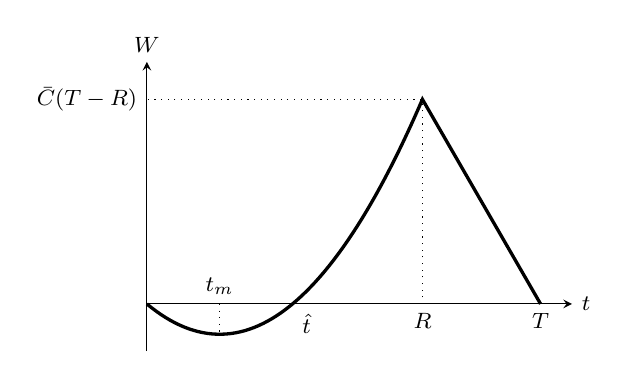
\begin{tikzpicture}[x=0.5cm,y=0.75cm,font=\footnotesize,>=stealth]
  \draw[->] (0,0) -- (10.8,0) node[right] {$t$};
  \draw[->] (0,-0.8) -- (0,4.1) node[above] {$W$};
  \draw[very thick,domain=0:7,samples=60] plot (\x,{-0.555*\x+0.15*\x*\x}) -- (10,0);
  \draw[dotted] (7,0) -- (7,3.465) -- (0,3.465) node[left] {$\bar C(T-R)$};
  \draw[dotted] (1.85,0) node[above] {$t_m$} -- (1.85,-0.513);
  \node[below] at (7,0) {$R$};
  \node[below] at (10,0) {$T$};
  \node[below right] at (3.7,0) {$\hat t$};
\end{tikzpicture}\\[2pt]
{\footnotesize Figure 8.1-1. Left: income (thick) and consumption (dashed). Right: wealth. Drawn for $Y_0=0.6$,
$g=0.3$, $R=7$, $T=10$, so $\bar C=1.155$ and $gR^2>2Y_0(T-R)$: the young borrow until $\hat t=3.7$, and wealth
peaks at $W(R)=3.465$.}
\end{center}

\intuicao{Saving is future consumption: the individual saves when income is above its lifetime average and dissaves
when it is below, so wealth is the running area between the income line and the flat consumption line. It is built
up over the working life and run down to exactly zero in retirement: the hump of Modigliani and Brumberg.}
\armadilha{The peak at $R$ uses $Y(R^-)\ge\bar C$, which $g\ge0$ guarantees. If $g<0$ and income falls to $\bar C$
before retirement, at $t_p=(Y_0-\bar C)/|g|<R$, wealth is concave on $[0,R]$ and peaks at $t_p$, while $W(T)=0$ still
holds. Nor should $W(t)\ge0$ be imposed: the book allows borrowing, and it is optimal when income grows steeply.}
\refbib{Romer (2012), \S8.1, pp.~365--368, eqs.~(8.1)--(8.6) (the discrete-time version: flat consumption, permanent
income, saving as income minus its lifetime average); Modigliani and Brumberg (1954).}
\checado{\texttt{check-4-8-8-1.py} verifies with sympy the lifetime resources, $\bar C$, both pieces of $W(t)$,
$W(R)=\bar C(T-R)$, $W(T)=0$, the borrowing condition, $t_m$, $W(t_m)$ and $\hat t<R$; numerically, that $W$ peaks at
$R$ for random $(Y_0,g,R,T)$ with $g\ge0$, that budget-neutral perturbations of the flat path lower utility (log and
CRRA $u$), and the values plotted in Figure 8.1-1. The solution manual agrees; it draws only the case $Y_0>\bar C$,
without early borrowing.}
